\chapter{总结与分析}
%
%实验中遇到的问题及解决方案,收获和思考:对算法的理解、优缺点的评价、算法的适用场景
%
通过本次实验,我深刻地体会到了基于Minimax、Alpha-Beta算法和Expectimax算法的区别。前两者适用的场景需要满足很强的假设,即每个智能体都
执行最优解。但是现实情况下,往往不是这样,如果此时仍然适用这两个算法,则会导致智能体“过于谨慎”,从而表现一般。例如对于图\ref{exp}的场景,
如果吃豆人认为幽灵会执行最优解,那么它将必死无疑,此时,为了尽可能地增加分数,最优解是“自杀”,因为这样能减少由于时间带来的扣分。但是,
如果这两个幽灵的行为是随机的,又或者甚至会刻意避开吃豆人,那么吃豆人实际上是可以获胜的。Expectimax算法可以很好的处理这种情况,幽灵
的行为特征可以由计算期望时的概率分配来刻画,如果行为是完全随机的,那么各行为的概率相同,如果总是取最优解,那么最优行为的概率总是1.

\begin{figure}[H]
    \centering
    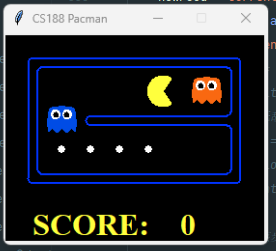
\includegraphics{./pic/sum.png}
    \caption{迷你地图}\label{exp}
\end{figure}

在实现算法时,还需要考虑的是所需的时间和计算量。为了降低开销,常常适用评估函数来进行估计,而非按照算法完成所有计算。虽然评估函数本质上是一个估计,
但是只要设计地足够好,便能够在降低开销的同时维持足够好的表现。在设计估计函数时,往往需要多次尝试。在本次实验中,我曾尝试用奖励项来激励吃豆人
主动收集能量点并追击幽灵、用惩罚项来让吃豆人避免进入死胡同等较不安全的位置,但事实证明,这些都可以用游戏得分来代替

在实验的过程中,遇到的问题集中在第5题。一开始吃豆人在某些情况下会停在最后一个食物旁边,但是一直不移动,直到幽灵靠近后才会开始移动。通过输出
日志的方式进行调试后,我发现问题在于当时我所设计的评估函数中,如果判断为获胜,则直接返回float('inf'),而在本题中,博弈树的深度限制在两层,
意味着吃豆人可以立刻移动至最后一处食物,从而游戏获胜,但也可以暂停移动一回合,然后再移动至最后一处食物,而这两种情况在博弈树的第一层中
都体现为float('inf'),如果解决平手的规则选择了暂停移动作为最佳行为,那么在幽灵靠近之前,吃豆人会一直保持静止。最后,我不再单独判断游戏失败或获胜,
因为这些都体现在了游戏分数之中,只需要在评估函数中包含游戏分数这一项即可。